%% Theorie.tex
%%
%\usepackage[ngerman]{babel}
%% ==============
\chapter{Theoretische Grundlagen}
\label{ch:Theorie}
%% ==============

{\bibliographystyle{babalpha-fl}}	% german style

Das Standardmodell der Teilchenphysik beschreibt die bisher bekannten Bausteine der Materie, sowie deren Wechselwirkungen. In Kapitel \ref{ch:Theorie:sec:Standardmodell} wird ein kurzer \"Uberblickblick dar\"uber gegeben, woraufhin in Abschnitt \cite{ch:Theorie:subsec:ttH} genauer auf die Produktion von Higgs-Boson und Topquark eingegangen wird.\\
Zur Untersuchung dieser theoretischen Vorhersagen, werden weltweit Experimente durchgef\"uhrt. In Kapitel \cite{ch:Experiment} wird das Compact Muon Solenoid (CMS) Experiment am Large Hadron Collider (LHC) des CERN vorgestellt. Um die dabei gewonnenen Daten auswerten zu k\"onnen, sind multivariate Analysemethoden notwendig. Diese werden in Kapitel \cite{ch:Theorie:sec:Algorithmen} behandelt, im Speziellen Boosted Decision Trees (Abschnitt \cite{ch:Algorithmen:subsec:BDT}).\\
Zum Vergleich verschiedenen Implementationen dieser Analysetechniken werden im Hauptteil dieser Arbeit statistische Methoden wie ROC Kurven verwendet. Diese werden in \cite{ch:Theorie:sec:statistischeMethoden} vorgestellt.

%% ===========================
\section{Das Standardmodell der Teilchenphysik}
\label{ch:Theorie:sec:Standardmodell}
%% ===========================

Der folgende Abschnitt soll einen kurzen \"Uberblick \"uber das Standardmodell der Elementarteilchenphysik geben, dabei bezieht er sich meist auf \cite{SWB-39819646X}.

Das Standardmodell der Elementarteilchenphysik fasst verschiedene Theorien der Teilchenphysik zusammen und vereinheitlicht diese.  Das Universum besteht aus einigen grundlegenden Bausteinen, die durch vier elementare Kr\"afte beeinflusst werden \cite{O'Luanaigh:1997201}. Die bislang beste Beschreibung dieses Aufbaus liefert das Standardmodell, wenngleich es die vierte Kraft, die Gravitation, nicht erkl/"aren kann. Dennoch war es mit diesem Modell m\"oglich fast alle experimentellen Ergebnisse zu best\"atigen, sowie sehr pr\"azise Vorhersagen \"uber verschiedene Ph\"anomene zu treffen.

Die bislang entdeckte Materie besteht aus zwei Arten von Elementarteilchen, den Leptonen sowie den Quarks. Diese lassen sich jeweils in drei Familien unterteilen. Jede Quark-Familie besteht jeweils aus einem Quarkpaar und deren Antiteilchen, diese sind Up- und Down-, Strange- und Charm-, sowie Bottom- und Topquark.\\
Leptonen bilden jeweils zusammen mit dem dazugeh\"origen Neutrino und den jeweiligen Antiteilchen eine Familie. Im Gegensatz zu den Quarks unterliegen Leptonen nicht der starken Wechselwirkung.\\
Die dritte elementare Wechselwirkung, die im Standardmodell beschrieben ist, ist die elektromagnetische Wechselwirkung. Ihr unterliegen alle geladenen Teilchen. Diese Wechselwirkungen sind in ihrer Struktur sehr \"ahnlich und werden durch den Austausch von Vektorbosonen vermittelt. Diese sind die Gluonen der starken Wechselwirkung, die W- und Z-Bosonen der schwachen Wechselwirkung und die Photonen ($\gamma$) der elektromagnetischen. 

Der letzte fehlende Baustein im Standardmodell ist ein elementares Spin-0 Teilchen, ohne das keine konsistente Erkl\"arung f\"ur die W und Z$^0$ Massen m\"oglich w\"are. Dieses ist das Higgs-Boson, welches 2012 am CERN entdeckt wurde. Die Kopplung zwischen Higgs-Boson und anderen Elementarteilchen ist proportional zur Teilchenmasse. In \cite{fig:Standardmodell} sind alle elementaren Bosonen und Fermionen dargestellt.

\begin{figure}[hhh]
 \begin{center}
   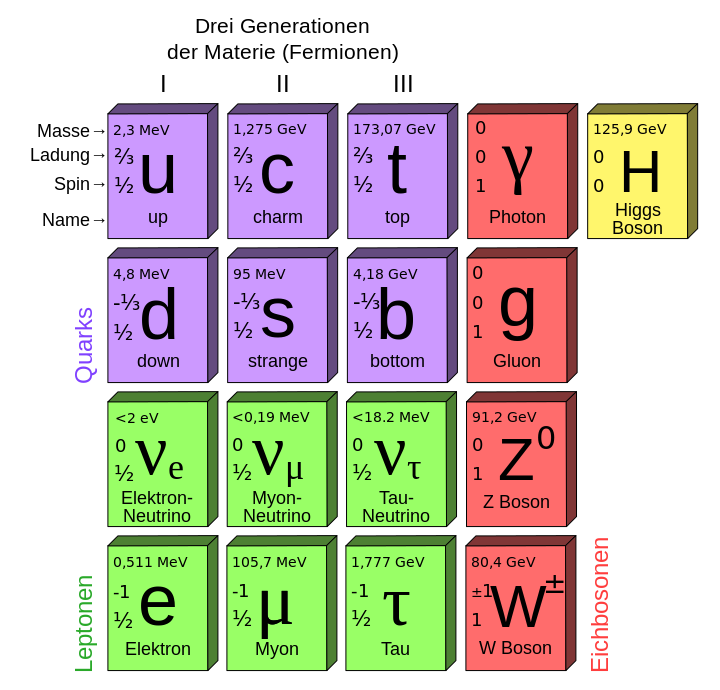
\includegraphics[width=\textwidth]{graphics/Standard_Model.png}
   \parbox[b]{12cm}{
     \caption[Standardmodell der Teilchenphysik]
             {\label{fig:Standardmodell} \it Die 12 fundamentalen Fermionen und 5 fundamentalen Bosonen des Standardmodells der Teilchenphysik,\\ Quelle: \cite{wiki:Standardmodell}}
   }
 \end{center}
\end{figure}

Insgesamt stimmen die experimentellen Ergebnisse gut mit den Vorhersagen des Standardmodells \"uberein. Dennoch reicht das Modell nicht aus, um s\"amtliche Ph\"anomene zu erkl\"aren. Im Modell werden beispielsweise masselose Neutrinos gefordert, allerdings ist durch die Neutrinooszillationen erwiesen, dass massive Neutrinos existieren.

%% ===========================
\section{ttH}
\label{ch:Theorie:subsec:ttH}
%% ===========================

%% ===========================
\section{Algorithmen zur multivariaten Analyse}
\label{ch:Theorie:sec:Algorithmen}
%% ===========================

Multivariate Analysemethoden bezeichnen Verfahren, mit denen, im Gegensatz zu univariaten Analyse statt jeder Variable einzeln, mehrere Variablen zugleich statistisch untersucht werden.\\
Aufgrund der sehr komplexen Problemstellungen ist eine Berechnung sehr aufw\"andig und daher manuell nicht zu bewerkstelligen. Mithilfe der zunehmenden Rechenleistung aktueller Computer ist dies jedoch m\"oglich und wird in vielen Bereichen immer wichtiger. Die Erforschung und Entwicklung dieser mathematischen Modelle bezeichnet man auch als maschinelles Lernen (machine learning), da mithilfe der Algorithmen versucht wird, aus Daten zu lernen und Vorhersagen zu treffen. \cite{SWB-455193959}

In der Hochenergiephysik nutzt man diese Methoden, indem man die Algorithmen, mithilfe der, durch theoretische Berechnungen erstellten, Simulationsdaten trainiert und anschlie\ss end die gemessen Daten klassifiziert.\\ 
Maschinelles Lernen spielt aber auch in vielen anderen Bereichen eine wichtige Rolle, wie beispielsweise im Finanzwesen, bei Studien zum Konsumverhalten, oder der Sprach-, Schrift- und Bilderkennung.

F\"ur diese Algorithmen existieren verschiedene Ans\"atze. Einer dieser Ans\"atze ist das \"uberwachte Lernen (supervised learning). Dabei wird anhand bekannter Trainingseingabewerte eine Klassifizierung der unbekannten Messwerte vorgenommen. Beispiele sind die St\"utzvektormethode, wobei jedoch die englische Bezeichnung support vector machine (SVM) gebr\"auchlich ist, Random Forest (RF), was Zuf\"alliger Wald bedeutet und mehrere zuf\"allig erstellte Entscheidungsb\"aume bezeichnet, oder Neuronale Netze. Ein weiteres Beispiel sind verst\"arkte Entscheidungsb\"aume (Boosted Decision Trees (BDTs)), die im Gegensatz zu Random Forests keine unkorrelierten Entscheidungsb\"aume nutzen.


%% ===========================
\subsection{Boosted Decision Trees (BDTs)}
\label{ch:Algorithmen:subsec:BDT}
%% ===========================

Entscheidungsb\"aume unterteilen den Bereich des zu klassifizierenden Objektes anhand gerader Schnitte auf desses Eigenschaften (Variablen) in mehrere Sequenzen. Wieviele dieser Sequenzen ab dem Wurzelknoten erstellt werden, wird durch die Tiefe (depth) des Baumes angegeben. In \ref{fig:DecicionTree} ist ein Beispiel eines Baumes mit der Tiefe zwei zu sehen.\\
\begin{figure}[hhh]
 \begin{center}
   \includegraphics[width=\textwidth]{graphics/tree.pdf}
   \parbox[b]{12cm}{
     \caption[Entscheidungsbaumes der Tiefe 2]
             {\label{fig:DecicionTree} \it schematische Abbildung eines Entscheidungsbaumes der Tiefe 2. X und Y sind die Variablen anhand denen durch cuts (Zahlen nach den Variablen) zwischen Untergrund und Signal unterschieden werden soll.\\Erstellt mit TMVA}
   }
 \end{center}
\end{figure}
Man unterscheidet zwischen zwei Arten, bin\"aren B\"aumen mit diskreten R\"uckgabewerten zur Unterscheidung mehrerer Klassen (classification trees), zum Beispiel Signal und Untergrund, sowie denjenigen mit kontinuierlicher Antwort (regression trees).\cite{SWB-455193959}

BDTs vereinen durch Boosting und Bagging (aus dem Englischen von bootstrap aggregation abgeleitet) mehrere Entscheidungsb\"aume zu einem starken Klassifikator.



%% ===========================
\section{statistische Methoden}
\label{ch:Theorie:sec:statistischeMethoden}
%% ===========================


%% ===========================
\subsection{Receiver Operating Characteristic}
\label{ch:Algorithmen:subsec:ROC}
%% ===========================


%% ===========================
\subsection{Kolmogorov-Smirnov Test}
\label{ch:Algorithmen:subsec:KSTest}
%% ===========================